% =====================================================================================
% REVISIÓN 2  -  Propuesta de solución
% Escribe tu texto FUERA de los recuadros \begin{guia} ... \end{guia}.
% =====================================================================================

\section{Propuesta de solución} \label{sec:propuesta} % audit:req=propuesta_solucion

\begin{guia}[Guía: Propuesta de solución (Revisión 2)]
\textbf{¿Para qué sirve?} Explica \emph{qué vas a hacer exactamente y cómo resuelve el problema}, antes de entrar a los
detalles de construcción (Revisión 3).

\textbf{Debe responder:}
\begin{itemize}[nosep,leftmargin=*]
  \item ¿En qué consiste la solución, a grandes rasgos? Incluye un diagrama general (arquitectura, flujo del proceso o
        esquema del método).
  \item \emph{Proyecto de sistema:} ¿cuáles son los requisitos funcionales (qué hará) y no funcionales (rendimiento,
        seguridad, usabilidad)? ¿quiénes son los usuarios y qué roles tienen?
  \item \emph{Proyecto de investigación:} ¿cuál es la hipótesis o pregunta de investigación? ¿qué enfoque o algoritmo
        propones y en qué se diferencia de lo existente?
  \item ¿Qué tecnologías, herramientas y metodología de trabajo usarás y por qué (frente a las alternativas)?
  \item ¿Cómo atiende la propuesta cada objetivo específico? (una tabla ``objetivo $\rightarrow$ componente de la solución''
        es muy útil).
  \item ¿Cuál es el plan de trabajo y el cronograma del cuatrimestre?
  \item ¿Cómo sabrás que funcionó? (criterios de aceptación o métricas de éxito).
\end{itemize}

\textbf{Organización sugerida:} \verb|\subsection| para \emph{Descripción general}, \emph{Requisitos} (o \emph{Hipótesis y
enfoque}), \emph{Tecnologías y metodología} y \emph{Plan de trabajo}.

\textbf{Extensión mínima:} 150 palabras, además de diagramas y tablas.

\textbf{Errores frecuentes:} describir solo tecnologías sin explicar la solución; requisitos vagos (``el sistema será
rápido''); propuesta desconectada de los objetivos; cronograma sin fechas.

\textbf{Cómo se revisa:} coherencia con el problema y los objetivos, viabilidad en un cuatrimestre y claridad técnica.
\end{guia}

% >>> ESCRIBE AQUÍ la propuesta de solución (con una \subsection por apartado) <<<

\subsection{Descripción general}

La propuesta consiste en desarrollar un copiloto web para consultar documentación técnica y procedimientos de planta mediante preguntas escritas en lenguaje natural. El sistema tendrá una arquitectura cliente-servidor: el usuario interactuará con una interfaz web construida con HTML, CSS y JavaScript; el backend recibirá la pregunta mediante una API desarrollada con FastAPI; y el agente coordinará la recuperación de fragmentos documentales, la construcción del contexto y la comunicación con un modelo externo de IA. La respuesta incluirá el texto generado, el estado de la operación y las fuentes disponibles para que el usuario pueda revisar el documento relacionado.

El flujo general de la solución se representa en la Figura~\ref{fig:arquitectura_propuesta}. El modelo externo puede ser Gemini o un modelo basado en \textit{Generative Pre-trained Transformer} (GPT). La información documental será proporcionada por el corpus preparado por el Integrante 1. En esta etapa, el componente de consulta conservará los metadatos de cada fragmento y podrá trabajar con el índice local de pruebas; la conexión con un almacenamiento vectorial persistente se dejará preparada para la siguiente etapa de integración.

\begin{figure}[htbp]
\centering
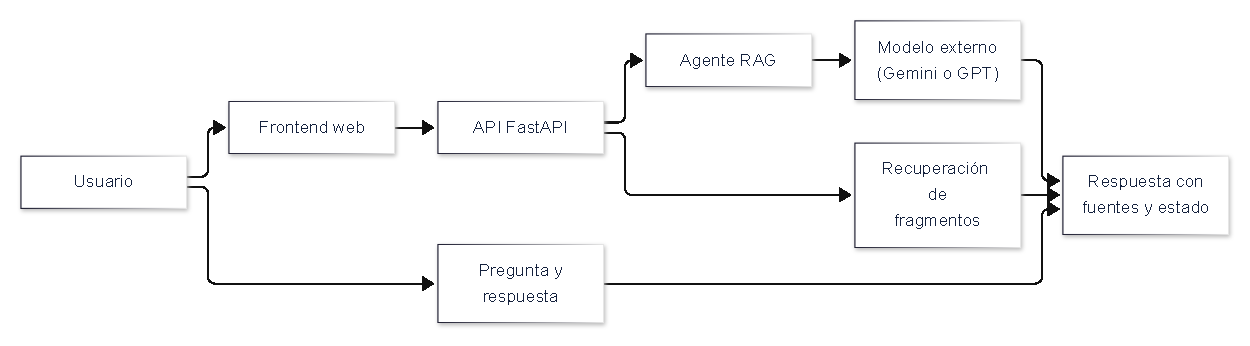
\includegraphics[width=\textwidth]{img/arquitectura_mermaid.pdf}
\caption{Arquitectura general propuesta para el copiloto documental.}
\label{fig:arquitectura_propuesta}
\end{figure}

\subsection{Requisitos funcionales y no funcionales}

Los requisitos funcionales describen las acciones que el sistema debe permitir al usuario:

\begin{itemize}
    \item Escribir una pregunta y enviarla al agente desde la interfaz web.
    \item Recibir una respuesta generada a partir del contexto documental recuperado.
    \item Mostrar el estado de la consulta, incluyendo respuesta disponible, falta de contexto o error del proveedor.
    \item Mostrar las fuentes relacionadas con la respuesta, incluyendo el archivo, la página o sección y la puntuación disponible.
    \item Abrir el documento citado desde la interfaz cuando exista una ruta válida.
    \item Consultar la biblioteca y cargar documentos permitidos para su preparación posterior, sin sustituir el proceso de ingesta documental.
    \item Devolver una respuesta de incertidumbre cuando la documentación disponible no respalde la pregunta.
\end{itemize}

Los requisitos no funcionales establecen las condiciones de calidad de la solución. La interfaz debe ser sencilla y adaptable a pantallas de computadora y dispositivos móviles. La API debe validar el contenido recibido, limitar el tamaño de los archivos y responder mediante JSON. Las credenciales del proveedor de IA deben permanecer en el servidor y nunca enviarse al navegador. El sistema debe conservar la trazabilidad de las fuentes, manejar errores de comunicación y permitir que los componentes puedan probarse por separado.

\subsection{Usuarios y roles}

El usuario principal es el personal que necesita consultar procedimientos, manuales o documentos técnicos de planta. Su función consiste en formular preguntas, revisar la respuesta y abrir las fuentes antes de tomar una decisión operativa. El responsable de documentación o administrador mantiene la biblioteca, verifica los documentos vigentes y supervisa la calidad de las respuestas. El responsable técnico mantiene la API, la configuración del proveedor, el índice de recuperación y los registros de prueba. La propuesta no autoriza al agente a reemplazar la aprobación de un supervisor ni a convertir una respuesta automática en una instrucción oficial.

\subsection{Tecnologías y metodología}

La interfaz se implementará con HTML, CSS y JavaScript para conservar una estructura sencilla y facilitar su mantenimiento. FastAPI se utilizará como frontera de comunicación HTTP, con modelos de validación para las solicitudes y respuestas, de acuerdo con las capacidades documentadas del framework \cite{fastapiDocs}. El flujo del agente se organizará mediante un grafo de estados con LangGraph y plantillas de prompt de LangChain, de modo que la recuperación, la decisión sobre la suficiencia del contexto y la generación queden separadas \cite{langchainDocs,langgraphDocs}. Gemini o GPT se considerará el proveedor externo de generación, seleccionado mediante una variable de entorno y no mediante una clave escrita en el frontend \cite{googleGeminiApi}.

La recuperación se realizará sobre los fragmentos y metadatos entregados por el Integrante 1. El índice local permite hacer pruebas reproducibles mientras se termina de definir el almacenamiento vectorial persistente; posteriormente podrá conectarse con PostgreSQL y pgvector sin cambiar el contrato de la API. El trabajo seguirá una metodología incremental: primero se valida la interfaz y la comunicación básica, después la recuperación y las fuentes, y finalmente la integración con el proveedor y las pruebas con preguntas representativas.

\subsection{Relación entre objetivos y componentes}

La Tabla~\ref{tab:objetivos_propuesta} muestra cómo cada objetivo específico se atiende mediante un componente de la propuesta.

\begin{table}[htbp]
\centering
\caption{Relación entre objetivos específicos y componentes de la solución.}
\label{tab:objetivos_propuesta}
\begin{tabular}{p{0.38\textwidth}p{0.49\textwidth}}
\toprule
\textbf{Objetivo específico} & \textbf{Componente que lo atiende}\\
\midrule
Facilitar la consulta de documentación técnica mediante lenguaje natural. & Interfaz web de chat y endpoint \texttt{POST /chat}.\\
Recuperar información relacionada con la pregunta. & Índice de fragmentos, búsqueda semántica y contrato de resultados con metadatos.\\
Generar respuestas sustentadas y trazables. & Agente RAG, prompt restringido al contexto y citas con enlaces a documentos.\\
Controlar respuestas sin evidencia suficiente. & Umbral de recuperación, estado \texttt{no\_context} y mensaje explícito de incertidumbre.\\
Mantener una base extensible para documentos nuevos. & Biblioteca de documentos, endpoint de carga y separación entre frontend, backend y corpus.\\
\bottomrule
\end{tabular}
\end{table}

\subsection{Plan de trabajo y criterios de aceptación}

El plan de trabajo se divide en etapas incrementales. En la primera se revisan los requisitos y se valida la estructura del corpus. En la segunda se integran la interfaz, la API y el flujo de consulta. En la tercera se prueban la recuperación, los metadatos y los enlaces a las fuentes. En la cuarta se realizan pruebas con preguntas que sí tienen respuesta en los documentos y preguntas externas al corpus. Finalmente, se documentan los resultados, las limitaciones y las tareas de continuación.

La solución se considerará funcional cuando una pregunta válida pueda enviarse desde el frontend y llegar al backend sin cambiar de ruta ni exponer credenciales; cuando el backend pueda devolver una respuesta JSON con estado; cuando una pregunta respaldada produzca fragmentos y fuentes consultables; y cuando una pregunta sin evidencia produzca una respuesta de incertidumbre sin inventar información. También se verificará que los errores del proveedor, los formatos no permitidos y los documentos inexistentes se comuniquen de forma comprensible al usuario.
